%----------------------------------------------------------------------------------------
%	PACKAGES AND OTHER DOCUMENT CONFIGURATIONS
%----------------------------------------------------------------------------------------

\documentclass[twoside, a4paper, titlepage]{article}

\usepackage{fancyhdr} % Required for custom headers
\usepackage{lastpage} % Required to determine the last page for the footer
\usepackage{extramarks} % Required for headers and footers
\usepackage{graphicx} % Required to insert images

% Margins
\topmargin=-0.45in
\evensidemargin=0in
\oddsidemargin=0in
\textwidth=6.5in
\textheight=9.0in
\headsep=0.25in

\linespread{1.1} % Line spacing

% Set up the header and footer
\pagestyle{fancy}
% \lhead{\docAuthorName} % Top left header
\rhead{\firstxmark} % Top right header
\lfoot{\lastxmark} % Bottom left footer
\cfoot{} % Bottom center footer
\rfoot{Page\ \thepage\ of\ \pageref{LastPage}} % Bottom right footer
\renewcommand\headrulewidth{0.4pt} % Size of the header rule
\renewcommand\footrulewidth{0.4pt} % Size of the footer rule

\setlength\parindent{0pt} % Removes all indentation from paragraphs

%----------------------------------------------------------------------------------------
%	TITLE PAGE
%----------------------------------------------------------------------------------------

\title{
  \vspace{2in}
  \textmd{\textbf{
    Imperial College 3rd Year Group Project \\
    Tracing and Identifying Cattle
  }}
  \vspace{3in}
}

\author{
	Frederick Lindsey, Thomas Szyszko \\
	Karim Nahas, Hongjiang Liu, Gregoire Yharrassarry
}
\date{9th January 2017}

%----------------------------------------------------------------------------------------

\begin{document}

\maketitle

%----------------------------------------------------------------------------------------
%	TABLE OF CONTENTS
%----------------------------------------------------------------------------------------

\tableofcontents

%----------------------------------------------------------------------------------------


\begin{section}{Executive Summary}
%------------------------------------------------------------------------------
% No implementation, software engineering details, or project management
%------------------------------------------------------------------------------

%------------------------------------------------------------------------------

\begin{subsection}{The Elevator Pitch}
  Advances in technology have revolutionised other industries and parts of agriculture, bringing with it radically improved methods and cost efficiencies. However, the methods used to identify, catalogue, and mark cattle have remained old-fashioned and out-of-date.

  Globally, with particular focus on developing countries, cattle are revered. They often represent a high proportion of a farmer's livelihood and wealth. It is in such countries where the systems required to protect a farmer's livelihood and his cattle are at their weakest and the greatest opportunity arises for corruption and theft of cattle.

  CowHub provides access to a catalogue of cattle which can be used to for identification purposes without the need for physical deformation of the animal. In doing so, any cattle that has not been tampered with (it's muzzle) can be identified as belonging to it's owner deterministically and with near certain reliability\footnote{Whilst no statistical tests have been performed during this project, previous works have indicated that the unique identity of a cattle is tied with the 'fingerprint'-esque nature of it's muzzle}.
  % TODO: Reference to paper regarding testing of 2,500 muzzles
\end{subsection}

%------------------------------------------------------------------------------

\begin{subsection}{Project Description}
  This project will focus on providing a technology-based answer to the problem aformentioned. It will consist of the development of a user-friendly platform that uses a scalable and centralised cattle management and identification system. The three key objectives for this project are the following:

  \begin{itemize}
  	\item Offer a \textbf{harmless, physically non-destructive alternative} to current methods used to identify cattle
  	\item Provide a service that \textbf{allows the identification of cattle}
  	\item Collect data on cattle from farmers to be able to \textbf{build and use a widespread catalogue of information regarding cattle and their movements}, relating to current and future (not yet foreseen) purposes.
  \end{itemize}

\end{subsection}

%------------------------------------------------------------------------------

\begin{subsection}{What is the need for the project?}
  The process of marking cattle can be incredibly painful, regardless of the age of the cattle, and is a controversial aspect of the identification process for animal rights activists. Being subject to this pain or witnessing its offspring being subject to this the pain can be highly traumatic for a cow. Members of the public feel so strongly about the issue that protests have been made where by members of the public have branded themselves, much to the disgust of onlookers~\cite{theguardian1}.

  Whilst branding itself is no longer carried out in the United Kingdom, current methods, including piercing a cattle's ears, are still in use today and are without animal-friendly competition. Often these forms of marking or identification are aided by RFID tags on collars, and potentially chips which are ingested by the cattle allowing the cattle to be scanned.

  \begin{figure}[H]
  	\centering
    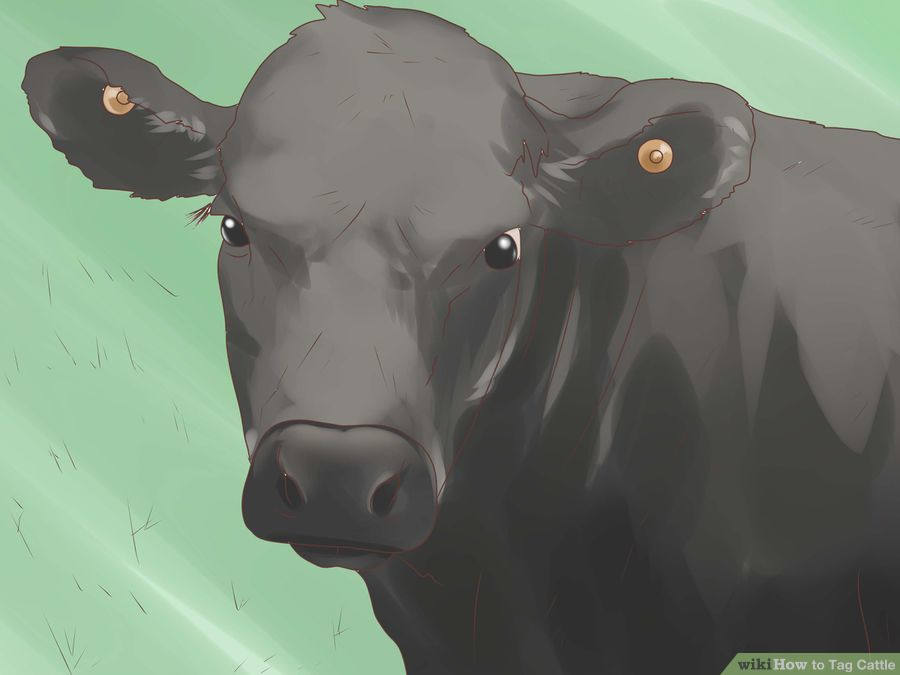
\includegraphics[width=0.5\textwidth]{images/cattle-with-ear-tag.jpg}
  	\caption[Cattle ear tagging]{
      Illustration of a cattle's head, demonstrating the position and rough size of cattle tags from the front. \cite{wikihow1}
  	}
  \end{figure}

  CowHub seeks to provide a user friendly platform to easily register and manage the information of a cattle. In addition, it also offers a non-intrusive solution for cattle recognition and by doing so alleviates all tagging-associated pain from implementing the current system.

\end{subsection}

\end{section}
% - Elevator pitch
% - What is the project? What does it do? What would I want to use/buy it?
% - No implementation, software engineering details, or project management


\begin{section}{Introduction}
There are around 300 million cattle worldwide. However the systems managing and tracking them varies significantly. Huge discrepancies between the procedures implement in developed and developing countries.

The EU has implemented a system of complete traceability from birth to death:
\begin{itemize}
	\item All cattle must have a unique identifier composed of the country code, herd mark, check digit and individual number.
	\item All cattle are tagged shortly after birth (one tag with the unique identifier on each ear). Newer tags contain RFID tags containing additional information about the cattle. 
	\item All cattle must have a bovine passport containing their date of birth, their breed and information on their genetic lineage.
	\item Registers of cattle herds must be maintained and regularly inspected.
	\item All cattle movements (both national and international) must be maintained in a digital database.
\end{itemize}

Additionally, ever since a BSE (mad cow disease) outbreak in 1997, each step in the food chain is scrutinized. From cattle to milk or burger, a database of all relevant information (health, origin, etc.) is maintained. This means any issues can be traced back to a farm, a particular cow, and batch of feed they were eating. These measures proved to be particularly useful during the horse meat scandal. Experts were able to trace back the problem from Findus products in the UK, through firms in France and Holland, back to two Romanian slaughterhouses. However, even with the stringent regulations aforementioned, some farmers still try to cheat the system for financial gain. Currently, there is no method to uniquely identify an animal without physical tags and thus prevent cattle identity usurpation.

On the other hand, in developing countries, many of these systems are lacking. Unlike in the developed world, agricultural workers make up between 50\% and 90\% of the population’s working force. Additionally, herds are usually composed of only a handful of cattle in contrast with large number of animal on industrialised farms. Due to the lack of capital investment and economies of scale, local authorities are often unable to implement robust regulation and enforce strict cattle tagging and tracking protocols. Currently, most official systems are quite ineffective and inefficient.
\begin{itemize}
	\item Governmental records are often handwritten note which are not standardised between regions.
	\item Farmers often do not use tags but rather cut unique notches of the cattle’s ears or even brand them to identify them.
	\item Police officers are quite lax and are sometimes bribed to ignore effractions of the law.
\end{itemize}

Nonetheless, Africa on the whole is undergoing a technological revolution. In terms of communication infrastructure, many countries are bypassing developing landlines and have already implemented robust 3G and 4G networks. Many people already own a smartphone. African countries are keen and have been trying to implement proper book keeping to open up access to valuable foreign export markets like the EU.

Thus, there is a true need for a system that can provide reliable identification. It could vastly improve the economic circumstances of many farmers and could help prevent public disease outbreaks. Also the current methods used for tagging infringe certain animal rights.  CowHub is exactly that - an alternative solution to the current protocols that have been widely used in the cattle industry. It has been designed to solve the following undesirable characteristics and issues of its predecessors:

\begin{itemize}
	\item \textbf{Inhumane}: tag needs to be physically installed (pierced) into the ear of the cattle
	\item \textbf{Inefficient}: registration and the production of tags is time-consuming
	\item \textbf{Unsafe}: tags, and other physical additions, can be easily removed, removing a farmer's only record of ownership of their cattle
	\item \textbf{Obsolete}: with contention from the public, the system has not been updated or reviewed in a significant period of time
\end{itemize}

CowHub introduces a new and modern way to get around the aforementioned issues. CowHub is able to identify a cattle by using its biometric features\footnote{The muzzle as of now.}. This approach is non-intrusive as as does not relly on any physically attachment such as a tag to recognize cattle. Also, the biometrics features used are unique and do not change over time. Biometric recognition techniques have been widely used to prevent fraud, enhance security, and curtail identity theft\cite{biometrics}. Thus, the identity and integrity of each individual is guaranteed to be preserved.

\end{section}
% - Set the scene ('motivation')
% - State the problem you're trying to solve ('objectives')
% - Summarise main achievements


\begin{section}{Project Management}
%------------------------------------------------------------------------------
% Planning
%------------------------------------------------------------------------------

\subsection{Planning}

The CowHub project started with very open-ended objectives, as seen above. Clearly, focused and specific planning was required. For the first week of the project we sought to narrow down exactly what this project meant and hoped to achieve, and the resulting week-long sprint proved highly successful and we realised the following:

\begin{itemize}
	\item We needed to delegate our responsibilities, between front-end interfaces and for back-end services
	\item The pivot point in our project would be a central, open API which would provide the backbone between our public and private services
	\item We needed to use stable, durable systems with sufficient amounts of compute power available, and link these with a solid continuous integration and deployment system
\end{itemize}

Owing to the abstract and preliminarily unidentified technical objectives of the project, a significant part of our team work and organisation has been to evolve the project description and iteratively redefine it. Consequently, we have seen various unanticipated changes in both infrastructure and 

%------------------------------------------------------------------------------
% Group organisation
%------------------------------------------------------------------------------

\subsection{Group Organisation}

In the beginning, the group members allocated each other responsibilities to give the project direction and a clear starting point for each member. As a group we decided on fundamental requirements for each component which was the only specification for each microservice / interface. The group agreed that we would spend as little time as possible in a horizontal development stage, and by parallelising the bootstrapping of the project, we were able to quickly reach a position where we could employ strong software engineering practices to maintain a high level of productivity. The responsibilities we each started with are below:

\begin{itemize}
	\item	\textbf{Frederick Lindsey, Gregoire Yharrassarry, Karim Nahas} \\
		  	Initial web front-end and basic API gateway, providing stateless session management, and performant asynchronous access to back-end services. 
		  	Bootstrapping the React-Redux web front-end and Ruby-on-Rails API gateway repositories. Setting up continuous integration and deployment for these repositories.
	\item 	\textbf{Thomas Szyszko} \\
		  	Investigated and implemented a portable mobile platform which could be used to input cattle information and identify cattle.
		  	Initialised and bootstrapped a Cordova-based application.
	\item 	\textbf{Hongjiang Liu} \\
	 	  	Researched and implemented an algorithm to process an image into keypoints used for comparison to provide functionality determining how similar images and their textures are.
	 	  	Extensive research into best practices for understanding images (machine-wise) and their differences.
\end{itemize}

As the project progressed, the responsibilities we each had became more and more general and translated across the platform. The group became very adaptable as the depth of each member's knowledge grew and we could all pick up any task on most components. The group had great flexibility when different members time constraints changed and was able to maintain a constant level of progress throughout the project resulting in a project that has been consistently worked on for three months. Crucial to this was meeting on a regular basis and maintaining persistent communication largely in the form of online communication and note-taking.

Towards the end of the project, due to time constraints, we reduced the breadth of the front-end footprint in order to focus on the core algorithm and infrastructure improvement to best achieve our directives and objectives.

%------------------------------------------------------------------------------
% Breakdown and task allocation
%------------------------------------------------------------------------------

\subsection{Breakdown and Task Allocation}

During the course of the project, the group experienced a myriad of changes to the way in which we managed ourselves and the tools we used. This allowed us to continually improve our productivity potential all whilst learning the ins and outs of real-world software engineering and development.

\subsubsection{Tracking tasks and issues}

Central to any software development is a teams ability to accurately, and in real-time, track what they are doing, what they need to do, and what they have achieved. The team adopted the Kanban approach, suggesting feature requests and issues onto a backlog, and dedicating resources to each task (often a user story) such that we maintained constant progress through the board. We used columns including 'Backlog', 'In Progress', 'Review', 'Done',  'Blocked' and 'Ignored' throughout our project to monitor tasks and be able to evaluate our performance as a team.

The first tool we tried to use to implement our chosen style of development was Trello \footnote{\href{https://trello.com}{Trello} provides an online workspace especially designed for todos and task management using cards.}

\begin{figure}[H]
	\centering
	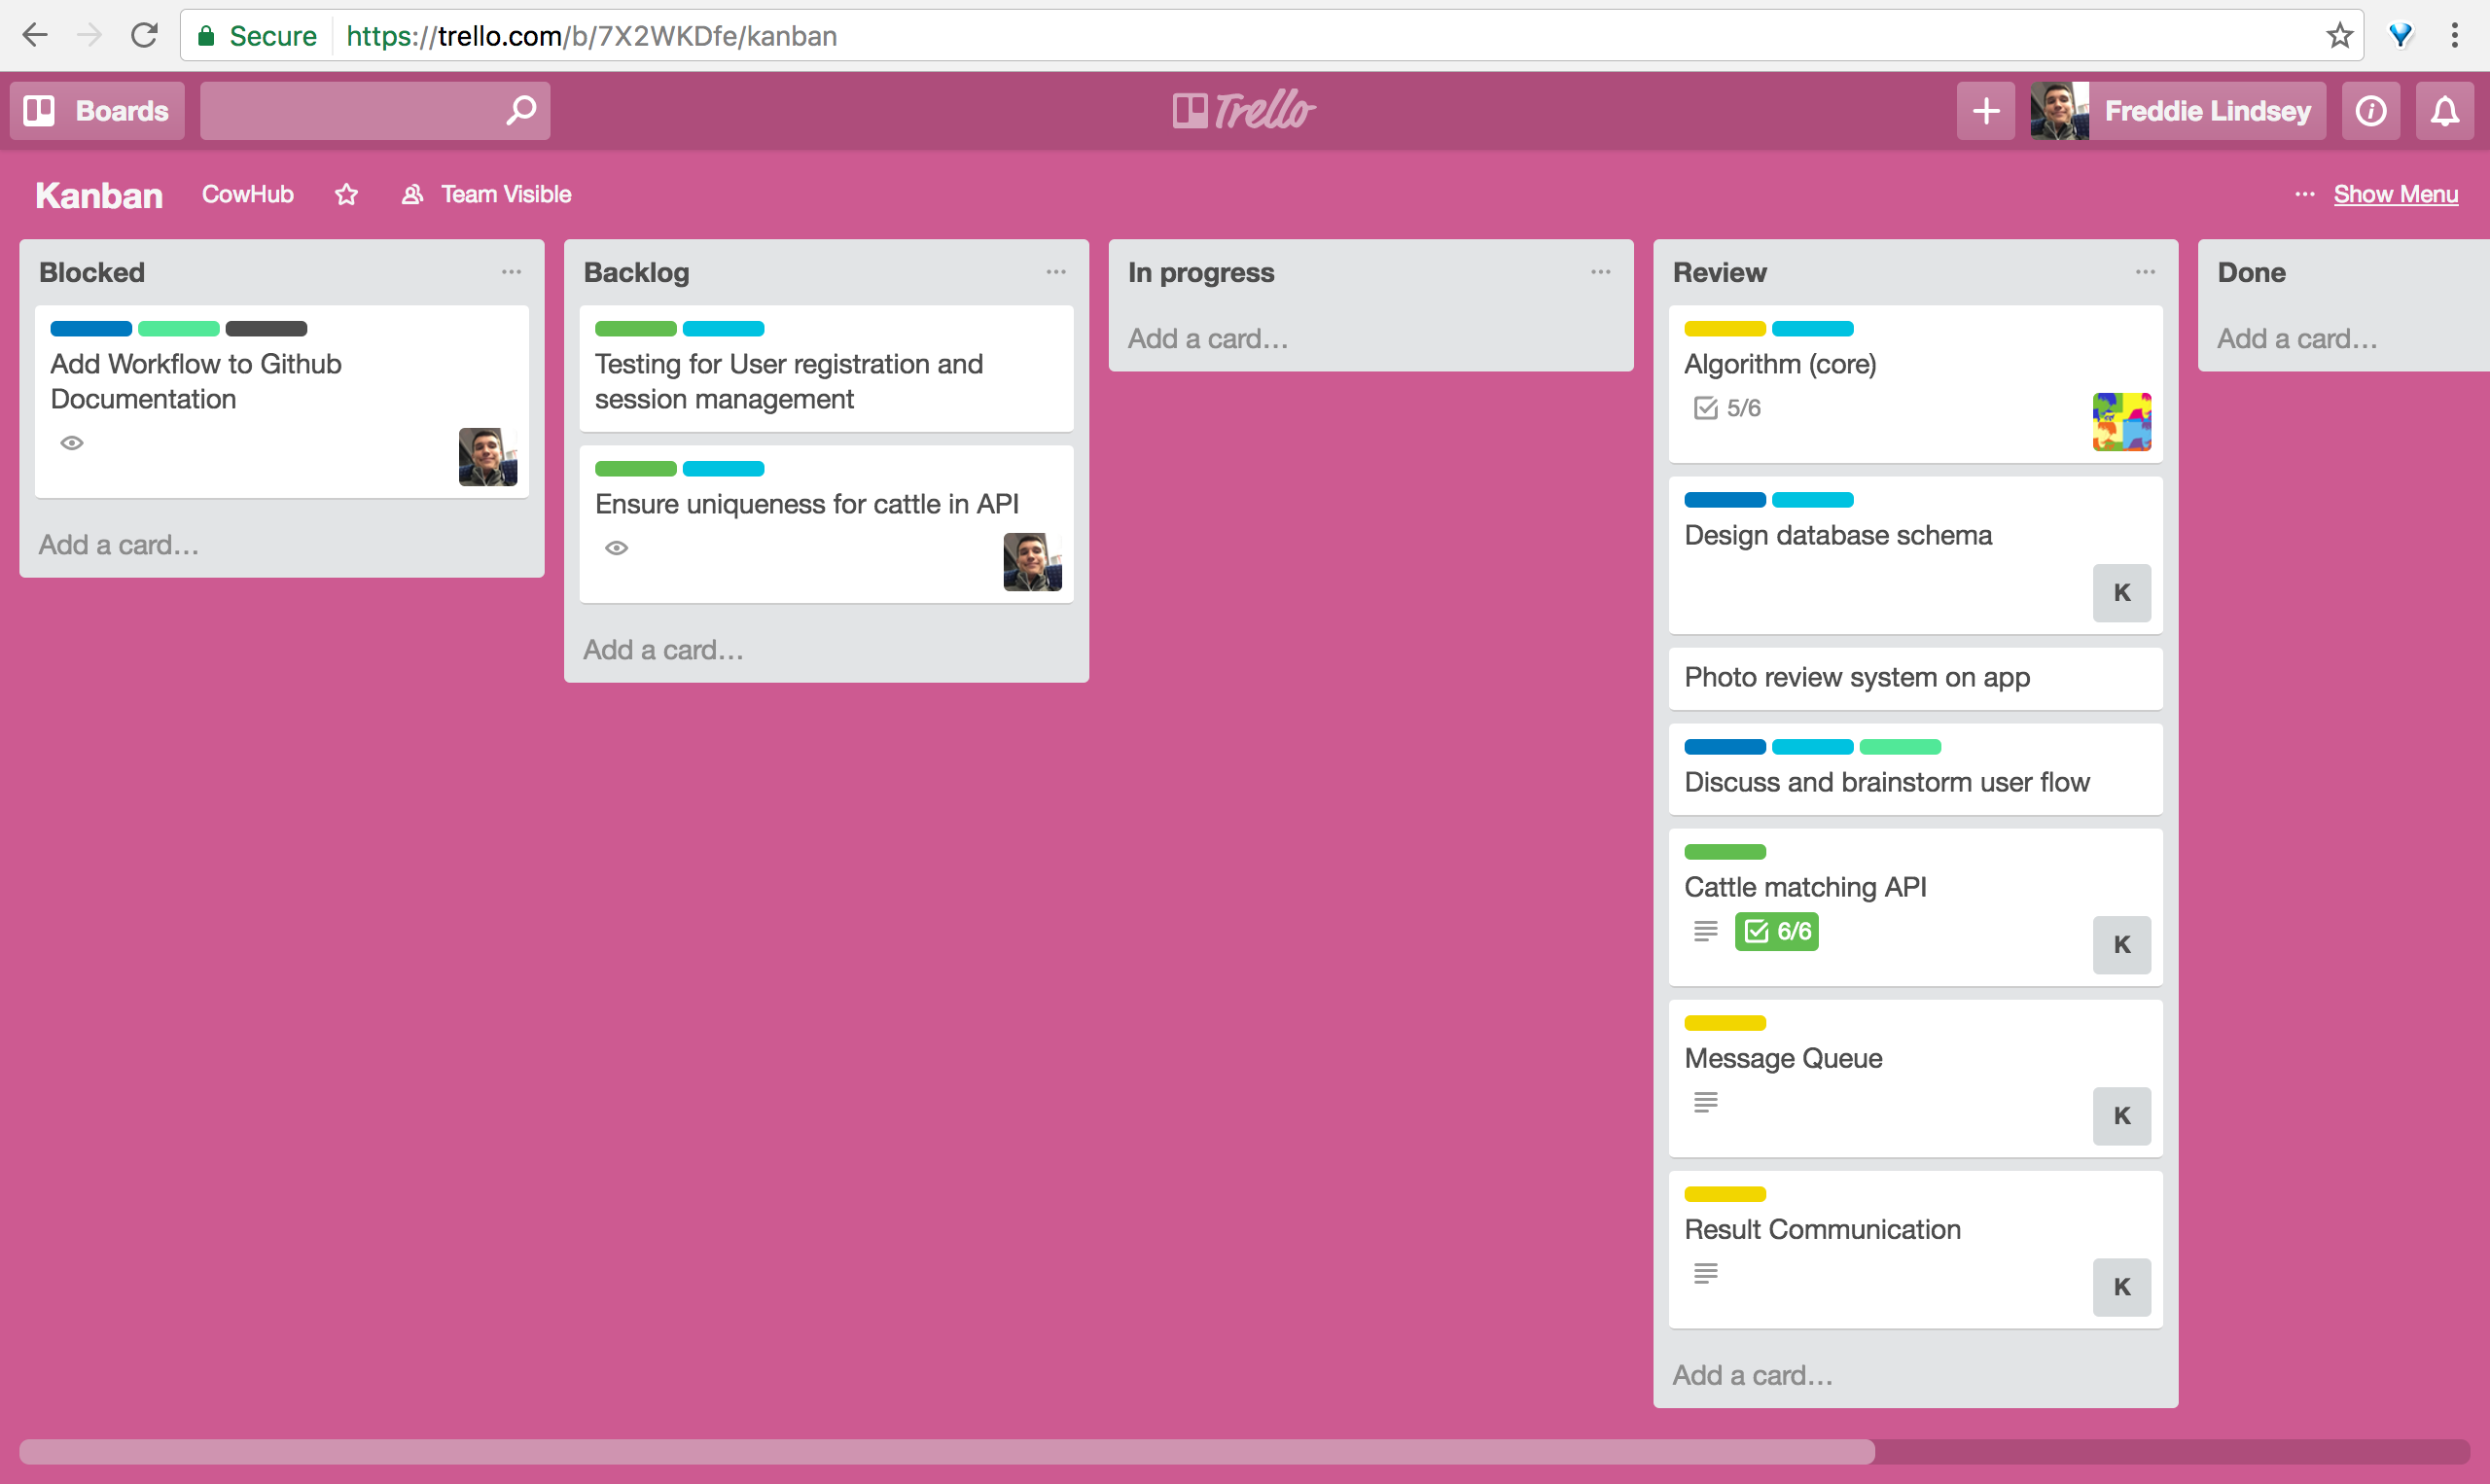
\includegraphics[width=0.8\textwidth]{images/trello-kanban}	
	\caption[CowHub's 'Kanban' board on Trello]{
		Our preliminary tool for tracking our tasks and issues, emulating the infamous Kanban approach.
	}
\end{figure}

During the limited time we chose to use Trello, we discovered that it made our development process more difficult, not easier as we had hoped and anticipated. 

\begin{figure}[H]
	\centering
	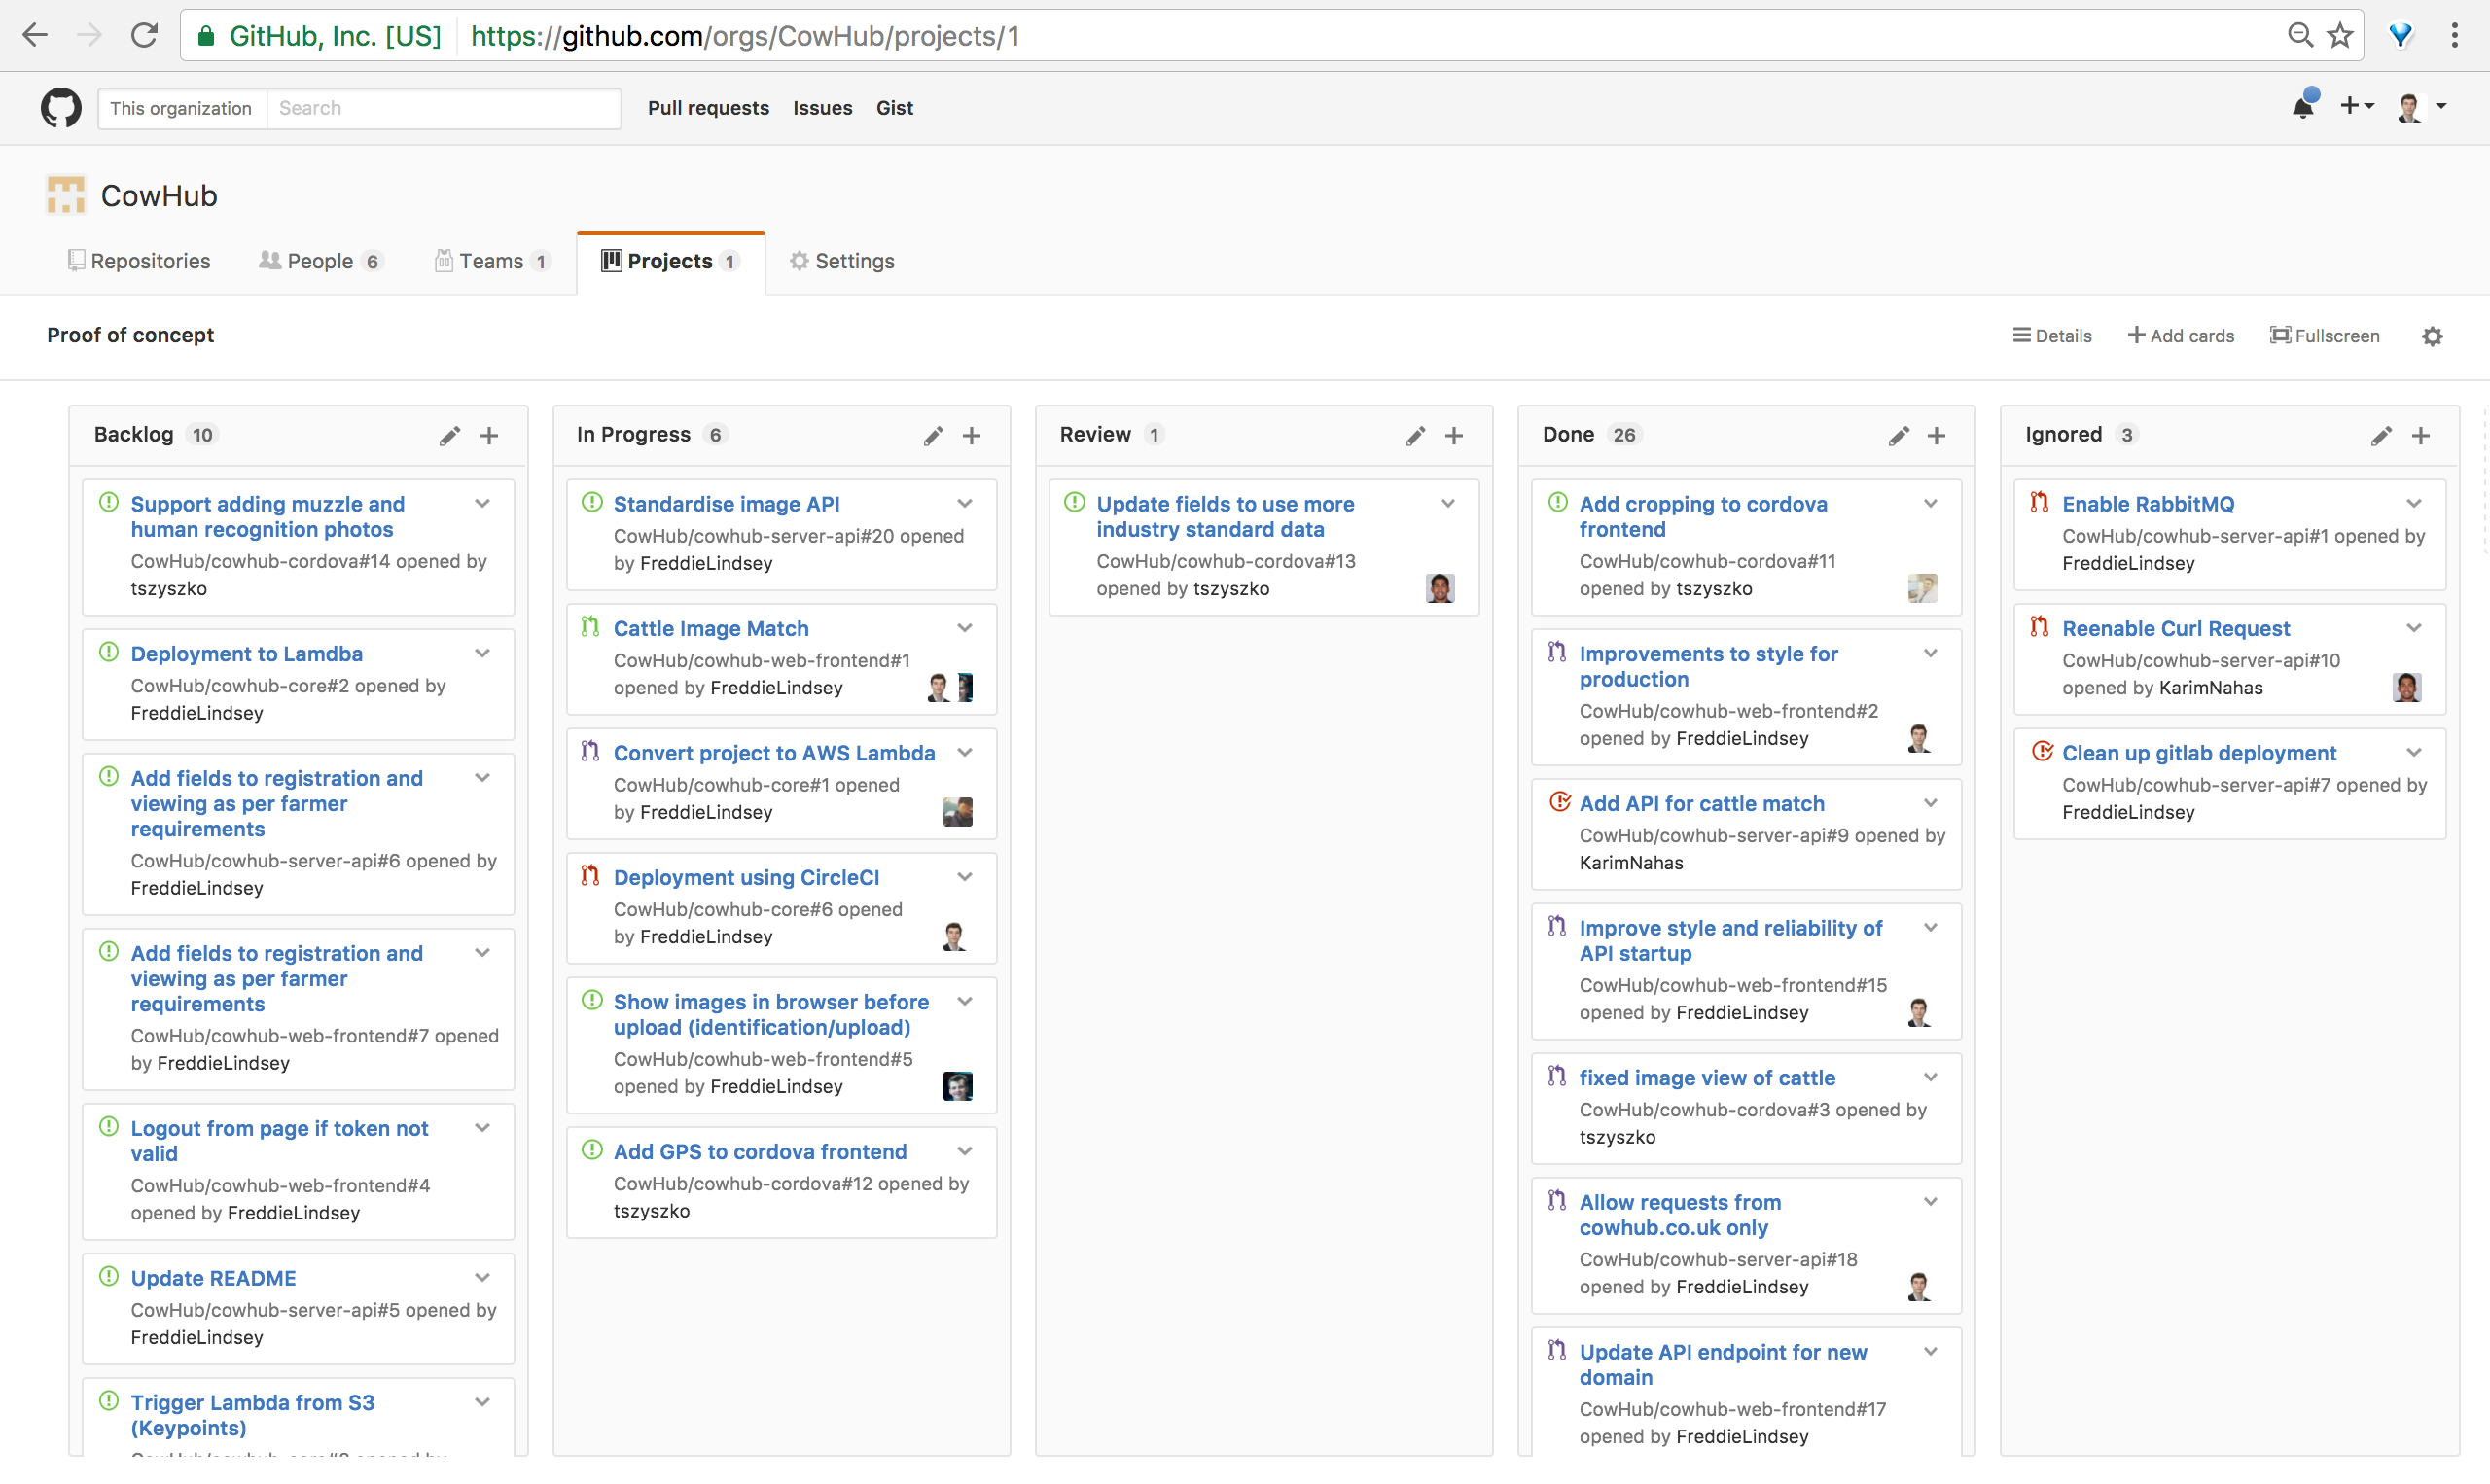
\includegraphics[width=0.8\textwidth]{images/github-project}
	\caption[CowHub's 'Kanban' board on GitHub using GitHub Projects]{
		A display of part of our board on GitHub, showing icons to determine the type of card
	}
\end{figure}


\subsubsection{Communication}








\end{section}
% - Planning
% - Group organisation
% - Breakdown and task allocation


\begin{section}{Design and Implementation}
CowHub, as opposed to being monolithic, has a number of small, modular components that serve different purposes and form a complete system. Each and every component is capable of running on its own, being built and tested independently and corresponds to a source repository on GitHub. For an overview of all important components, see Figure \ref{fig:structure}.

\begin{sidewaysfigure}
  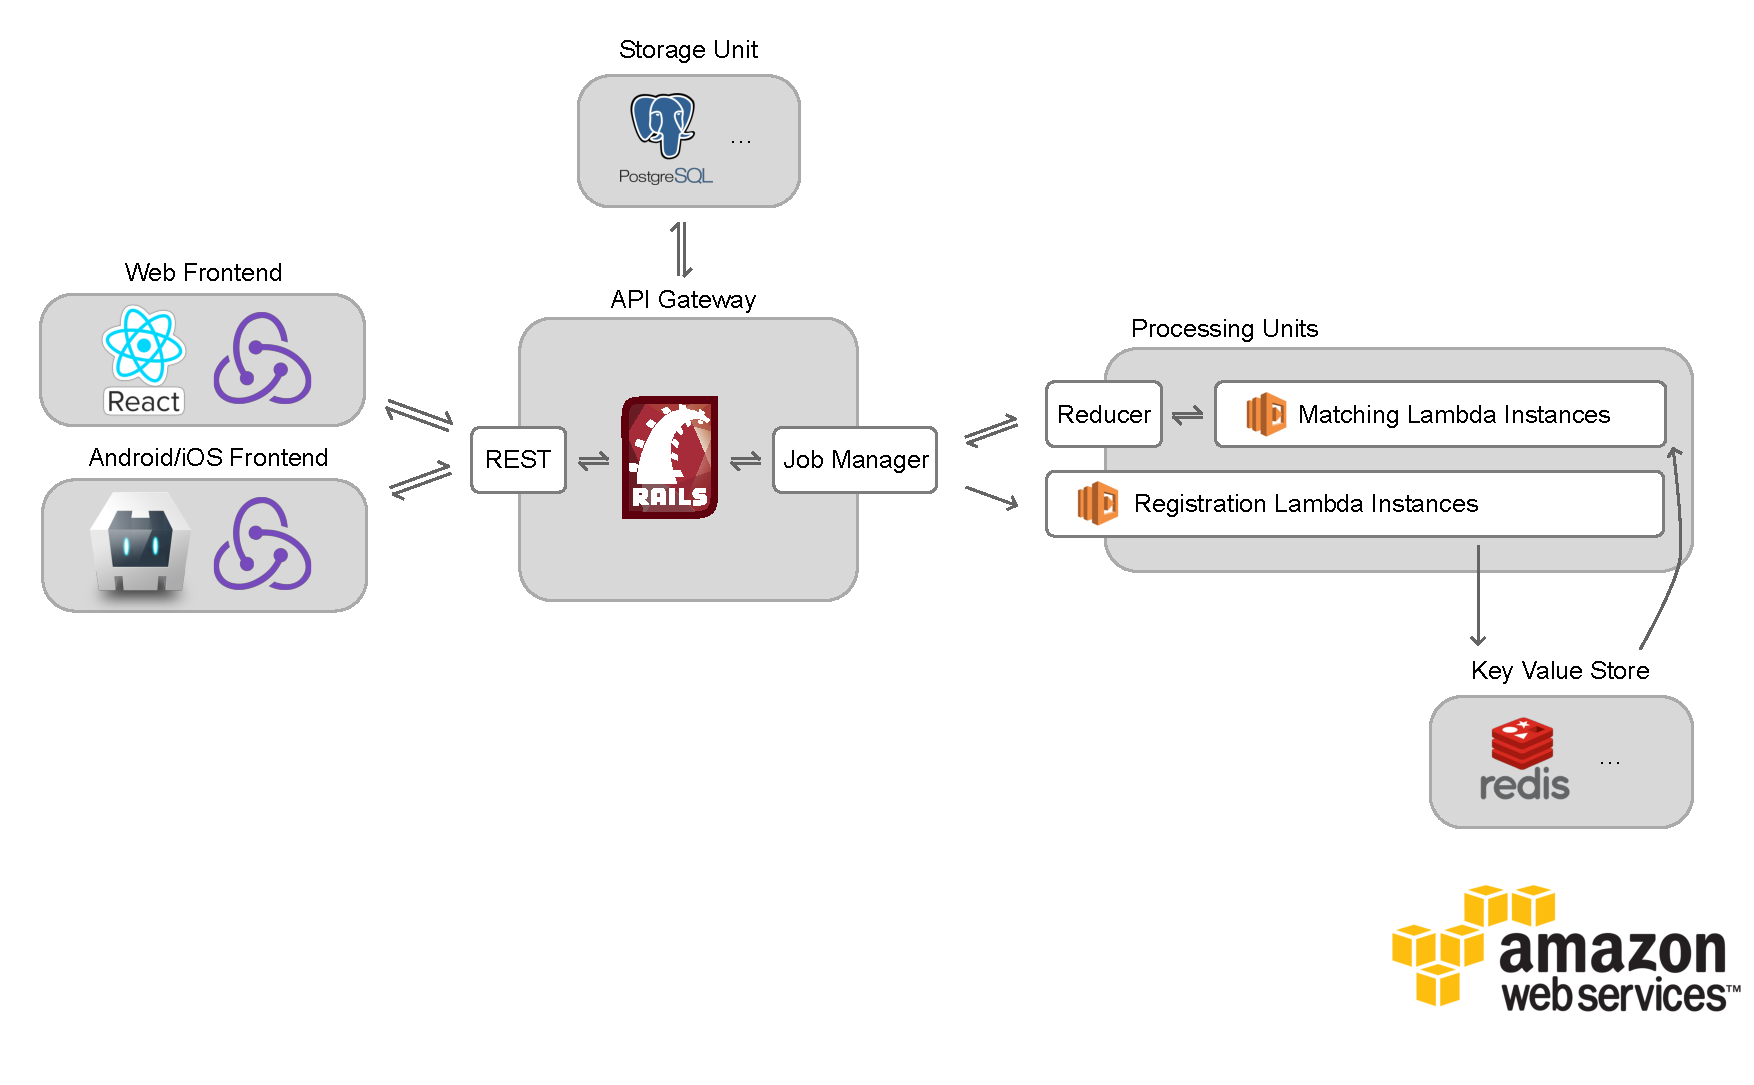
\includegraphics[width=\textwidth]{sketch/structure.pdf}
  \caption{The structure of CowHub}
  \label{fig:structure}
\end{sidewaysfigure}

CowHub employs Amazon Web Services (AWS) for a scalable, robust and stable cloud solution. For this project, the used services include IAM, CloudFront, Route 53, EC2, S3, RDS, Lambda, ElastiCache and API Gateway\footnote{This will later be referred to as Amazon API Gateway for disambiguation.}. The use of each service will be explained further in the following report.

The report proceeds with respect to the components of the project.

\subsection{Persistent Data Storage}
The database unit is built on top of Amazon Relational Database Service (RDS) and Amazon Simple Storage Service (S3), and PostgreSQL has been chosen to be the engine of the database service. The database unit aims to provide a simple, scalable and cloud-based database interface for our other services to use. 

RDS has been chosen because it is an easy solution to a resizable and scalable database, and provides features such as duplication. By employing RDS we could focus more on the application that we are building and pay little to no attention to the time-consuming database administrative tasks.

S3 is used to hold the image uploads. It has been chosen because of its simplicity to use, durable infrastructure and more importantly, its integration with other Amazon and CowHub services.

The database is to store the following:

\begin{enumerate}
	\item The information about farm and farmers. 
	\item The information about registered cattle, including the herd number, (optionally) the name, the owner, the birthdate, and most importantly the sample image(s) of its muzzle for identification uses.
	\item The login details of registered farmers. Farmers will need to log in to be able to input and review the cattle data.
	\item The match results. Every match job will be assigned a job ID and the result will be stored into the database. These match results will be useful in the future as statistics.
	\item Other data for the system to run smoothly (including session tokens etc.). 
	% TODO: more stuff about databases
\end{enumerate}

The database unit is only accessible through the API Gateway\footnote{Images are encoded in Base64 format before transfer (as a string).}.

\subsection{API Gateway}
The API Gateway (API) can be thought of as the centre of the system, and is written in Ruby on Rails (RoR). RoR has enabled us to prototype and implement the component in an elegant and efficient manner; its seamless integration with Rspec has also allowed us to test the component more efficiently\footnote{Nearly all sub-components have automated tests and are integrated with the continuous integration and delivery system.}.

The API has two most important subcomponents:

\begin{enumerate}
	\item A REST API for communication with the front-ends.
	\item A Job Manager for communication with the headless computational unit.
\end{enumerate}

The REST API mainly handles the following:

\begin{enumerate}
	\item Account management. A user (farmer) needs to be able to manage his/her personal data, change passwords and etc.
	\item Cattle management. A user (farmer) needs to be able to create/edit/delete information about a cattle and upload/update/delete images for a cattle. 
	\item Session management. The API handles sessions through tokens in a unified manner for all front-ends that require user login as REST API is stateless.
	% TODO: more stuff about our API
\end{enumerate}

We have a standardised URL schema for the API that allows us to develop the component more efficiently.

The Job manager is the more interesting part. There are two different types of jobs:

\begin{enumerate}
	\item Cattle registration job. For this type of job, an anonymous job is created (the result is not saved into the database). This is required because we do not match image with image; instead we used an edge descriptor to mathematically describe the muzzle of a cattle. The registration job is to deal with the descriptor generation so that we do not have to calculate the descriptor every time it is required.
	\item Cattle matching job. A job ID is required for this type of job as 1) we need to be able to track the status of the ongoing job and 2) we need to save the match result for statistical purposes. The process, roughly, includes (in the following order):
	\begin{enumerate}
		\item Generate the descriptor for the image to be matched.
		\item Divide the database of images into chunks with size $N$\footnote{A predefined value. For the proof of concept we have chosen 25.}, label each chunk with an ID $\text{id}_i$.
		\item For each chunk with ID $\text{id}_i$, forward the ID, the job ID and the image descriptor to the headless computational unit and wait for a best match within the chunk to be handed back. The headless computational unit will run asynchronously for all calls.
		\item Aggregate the result for a best match. Write the best match into the database and return it to the caller.
	\end{enumerate}
\end{enumerate}

Based on our statistics, step (a) normally takes a half to one second, and every pairwise match in step (c) takes about 30 to 80 milliseconds\footnote{This is due to the resizing and normalisation done prior to the match.}. That is, ignoring the network and IO delays, a match will take about $T = N * t_m / 1000 + t_d / 1000$ seconds to complete, where $t_m \in [30, 80]$ and $t_d \in [500, 1000]$. In this reasoning our computation time can be thought of as upper bounded by $Nc$, where $c \in \mathbb{Q}$, which is totally size-agnostic, because it is based on the assumption that we would always have $\lceil M / N \rceil$ computational units at our disposal. This rational implies that, in theory, the computation time does not generally grow with respect to the number of images in our database\footnote{In practice it does - because we cannot ignore the time consumed for IO actions.}.

\subsection{Key Value Store}
A cluster of Redis servers is employed through Amazon ElastiCache service. 

For performance reasons it has been decided that we use a key value store for concurrent and lively access for the descriptor of an image. This store is to be accessed very frequently and as only a small piece of data is being extracted at once it seemed inappropriate to be using a database. Another reason that a key value store is used, as opposed to accessing the descriptor directly from the database unit is data separation - the only place that this data is being accessed is the headless computational unit and nothing more. Also, as suggested before, the database unit is only accessible through the API, and any access directly from other components would break the promise; alternatively, to access the descriptors through the API would introduce significant (and unnecessary) burden to the API itself and result in great performance problems.

\subsection{Headless Computational Unit}
The processing is built on top of AWS Lambda services. The headless computational unit supports two different kinds of jobs: registration and matching, as suggested before. A call to the headless computational unit will cause a Lambda calculation unit (Lambda) to be spawned. Lambda processes are running concurrently, and they are not necessarily on the same machine\footnote{It can be thought of as Actors - universal primitives for concurrent computation. Similar constructs implementation include \textit{Akka} for Scala.}.

The two different kinds of the Lambda processes include:

\begin{enumerate}
	\item Registration Lambda. This is a one way communication. The caller (the API) calls the headless computational unit, causing a Registration Lambda to be spawned. This Lambda process will run to the end (the generation of the descriptor of an image) and then store it into the Key Value store.
	\item Matching Lambda. The caller will need to call the headless computational unit with the job detail, and the Matching Lambda will run the match for $N$ images as discussed before. This process is running concurrently. Upon finishing the process, the Lambda will forward the best match within a batch of $N$ images back to the caller as notification.
\end{enumerate}

The process of matching is similar to that of Map Reduce, and so is the implementation. The only difference, through the use of AWS Lambda, is that we do not provision or administer the servers ourselves - the computational units are spawned ad hoc and only whenever needed.

\subsection{Mobile and Web Front-ends}
Our mobile application supports Android and iOS platforms. There is no plan on supporting Windows Phone in the foreseeable future.

To assist the development process in a rather short period of time, we have decided to use a cross-platform solution to build our app on. More specifically, we have employed Apache Cordova framework as the foundation block of our app, and most of the application level programming is done in JavaScript. This implies that our apps have the so-called ``hybrid'' structure where

\begin{itemize}
	\item the interface prototyping is done in a unified manner, in JavaScript and styling in CSS - meaning that it will produce the same layout across different platforms because the interface is shown through a WebView\footnote{An important assumption made here is that the WebView will behave uniformly for the subset of layout techniques that we have used. Thanks to the use of WebKit rendering engine on both platforms and the standardised protocols and guidelines for the Web this assumption can be, to a degree, thought as true.};
	\item most of the higher level logic is written in JavaScript, giving the same behaviour cross-platform, meaning that we can start the development without any prior platform-specific knowledge;
	\item agile development of the application is allowed as there is little to none compilation required for the application to be built;
	\item most of the Node.js libraries are made available for use: React.js and Redux, for example;
\end{itemize}

The use of the the ``hybrid'' structure also yields certain disadvantages compared to developing the application natively. For example, the performance will, to some extent, suffer from the extensive use of WebView, and so will the battery life; access to low-level and platform dependent features are limited, and requires more fiddling\footnote{Normally through the native interface of the framework.} for it to work. But clearly for the amount of time given, and the state of the framework those disadvantages are out-weighted by the advantages listed above.

The Web front-end is coded using React.js and Redux, and there is no server side rendering required. For our Web front-end to work there only needs to be a server serving static files, thus making our Web front-end highly performant and scalable.

The front-ends are all stateless.
\end{section}
% - Detail of design
% - Summarise key implementation details
% 	- How did you do it?
% 	- What technology was used and why?


\begin{section}{Evaluation}

\subsection{Bootstrap and Lifecycle}

The different components of the system runs independently from each other. However, still, connection needs to be established to form the whole system. The said connections are not created eagerly, though, as to avoid the looping issues with (possible) cyclic dependency and to reduce the bootstrap time.

For the front-ends, as they are only created when needed, they do not to fit in the bootstrap stage. They will be able to work fine as long as the system is online at the time of use.

The structure of the system suggests the explicit dependencies of the system:

\begin{itemize}
	\item The API is dependent on the Persistent Storage as the API does not hold any data at the time of bootstrap.
	\item The API and Lambda depend on the Key Value Store.
\end{itemize}

and the implicit ones:

\begin{itemize}
	\item S3 should be present whenever API and Lambda is available as it serves as a mean to invoke the Lambda instances for the API.
	\item We have used the Redis (Key Value Store engine) Channel for Lambda state monitoring.
\end{itemize}

Topologically a reasonable bootstrap order, then, would be\footnote{That is, we sort the items based on a order that takes the dependencies into consideration. For more information regarding topological sort please see https://en.wikipedia.org/wiki/Topological\_sorting.}.

\begin{enumerate}
	\item[1] Persistent Storage Unit
	\item[1] Key Value Store
	\item[2] The API
	\item[3] Lambda\footnote{Lambda is quite special in terms of lifecycle. See below for detailed information.}
\end{enumerate}

where the order of items with the same number are inter-exchangeable.

Different components behave in different manners, in terms of its lifecycle:

\begin{itemize}
	\item The API resides inside Docker running on EC2. The actual deployment, scaling and provisioning are done through AWS Elastic Beanstalk~\cite{beanstalk}. We have also assumed that unless under special cases such as necessary offline maintenance or system upgrading, the service will not be offline. AWS Beanstalk will automatically re-boot the API if, under exceptional circumstances, the API goes down.
	\item The nature of persistence of the API naturally requires the persistence of the Persistent Storage Unit and Key Value Storage. Fortunately, due to the use of AWS RDS, S3 and ElastiCache there is no need for manual management of the components lifecycle.
	\item Lambda is a special type of unit. Lambda instances are only fired up whenever there is a cattle registration or match request coming in, and will be instantly destroyed/disregarded when the computation is done to save the resources. Lambda instances then have a very short lifecycle, and are fairly lightweight to bootstrap\footnote{In fact the bootstrap of each Lambda instance only requires the the connection to the Key Value Store. This process takes little to no time as they both are close both geographically and in the network.}.
\end{itemize}

Unfortunately, under certain cases, the services might have to be shut down. The order of shut down is rather different compare to that of bootstrap:

\begin{enumerate}
	\item The API needs to be notified first, as to stop accepting new requests.
	\item If there are running Lambda instances, wait for them to run to finish. This is acceptable as Lambda instances are programmed as lightweight computational units and generally a very small (~15 seconds) running time limit is imposed on all Lambda instances.
	\item The Persistent Storage Unit.
	\item The Key Value Store. However, extra care must be taken in the shutdown process of the Key Value Store to keep the data. Fortunately it is being backed up daily and at time of shutdown automatically.
\end{enumerate}

\subsection{Use of ElastiCache}

Unlike the name suggests, ElastiCache is not employed as a cache engine from a programming point of view, because we have assumed that the saved key-value pairs will always be available unless otherwise indicated. In our design the system uses Redis, the Key-Value storage to store the descriptors to reduce the running time of the matching process - a suggestion of, from a philosophical point of view, a caching process.

From the previous subsection it is pointed out that the data in the key-value store is being kept. This is not the ideal use case of any cache engine; however, in the future iterations, it has been agreed on that the system will handle the cache miss should it ever happen as a way to make the system more robust.

\subsection{Use of S3}

Our system has been using S3 extensively. There are two main uses for S3:

\begin{itemize}
	\item Image storage: images of cattle are saved onto S3. The index include the cattle ID and the image ID. User ID does not constitute part of the key as a cattle does not belong to one and only one owner.
	\item Action trigger. Object creation/update and deletion on S3 turns out to be able to send a notification message to the other Amazon cloud services.
\end{itemize}

One reason that S3 has been used as a simple action trigger service is that as it turns out, S3 has a much more robust connection with the rest of the Amazon Cloud services. The original implementation of the Job Assignment Lambda invokes the Matching Lambda with the official AWS SDK \texttt{boto3}, however that seemed to be unusable. The Job Assignment Lambda has a running time limit of 10 seconds, however the invocation process using \texttt{boto3} alone frequently bring the whole process to timeout\footnote{Our speculation is that it might be the \texttt{Payload} data that we are sending is over 500KB - a scenario that \texttt{boto3} is not optimised for.}. After some testing and digging around, we found out that if we save the parameter (the descriptor for the image to be matched against) onto S3 as an object, and if that triggers the invocation of the Matching Lambda, the problem would be resolved and it is lightning fast and there never had been any connection issues. We have decided to keep using S3 since after some debate for the non-ideal use of the service.

\subsection{Algorithm Performance}
\label{sec:algorithm}

It has been briefly discussed about the algorithm performance and the discussion will resume at this section. Note that the following tests are concluded on a machine with the

\begin{itemize}
	\item Processor: Intel Core i7-6820HQ, 2.7 GHz, 4 cores, 8 processes
	\item Memory: 16 GB 2133 MHz LPDDR3
	\item Operating System: macOS 10.12.2 (build 16C67)
\end{itemize}

and GPU acceleration turned off.

A simple test (with a sample size of 144 pairwise image matches) yields the following result, note that the edge and descriptor generation are for two images (unit: ms):

\begin{center}
\begin{tabular}{c|c c c}
        & Edge Generation & Descriptor Generation & Matching \\
\hline
Mean    & $135.20$       & $482.91$              & $47.15$  \\
Medium  & $136.68$       & $450.11$              & $42.77$  \\
SD      & $11.87$        & $91.72$               & $28.79$
\end{tabular}
\end{center}

Note that edge and descriptor generation are only done once for each request. The total time then is bound by the formula $N * t_m + t_d$ where $N$ is a fixed number, ignoring the time for IO actions. The running time is not upper bounded by the data size even though the matching process is essentially pairwise as an important assumption we have made is that we always have as many Lambda instances at our disposal as we want by our design.

An box-plot visualisation of the data is shown in the combined plot ~\ref{fig:algo_visual_all}.

\begin{figure}[H]
	\centering
	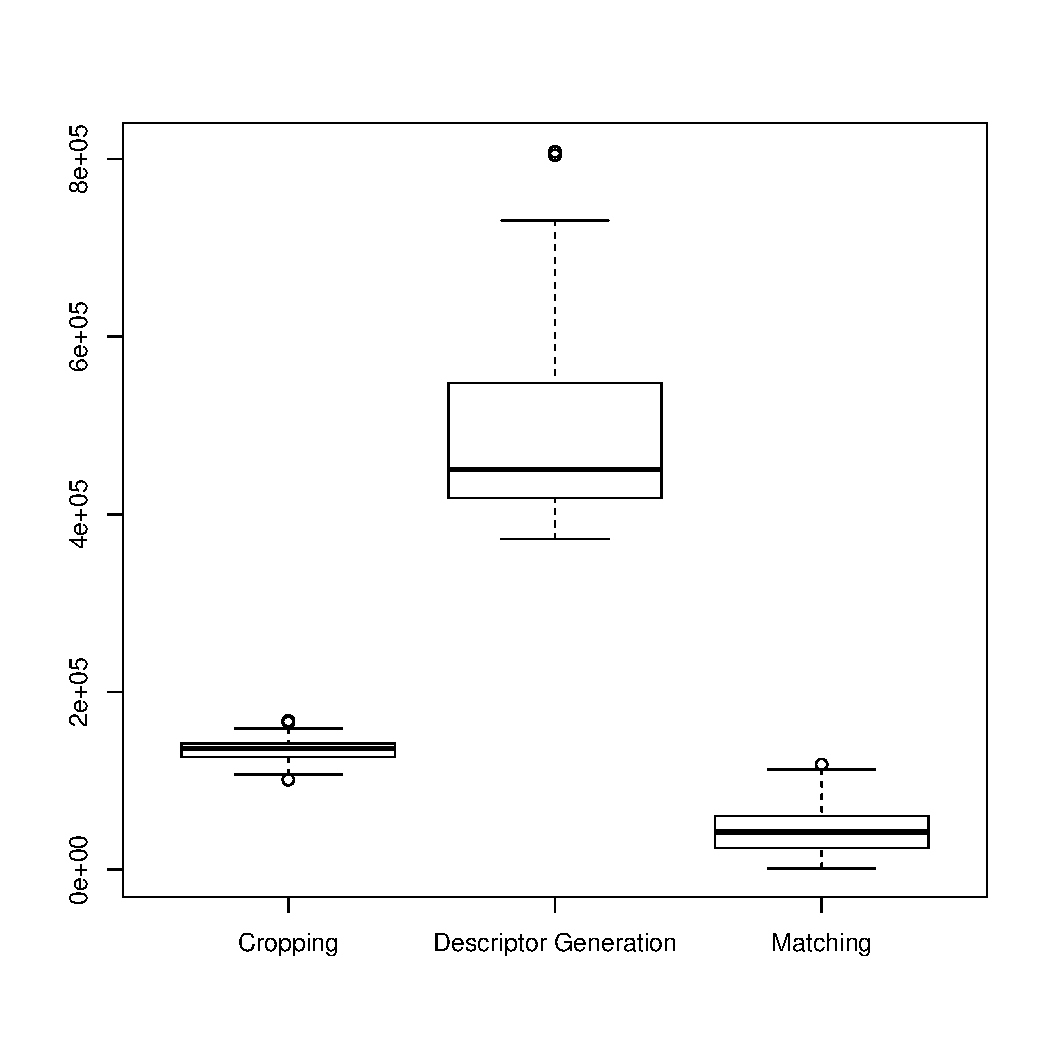
\includegraphics[width=0.8\textwidth]{sketch/all.pdf}
	\caption{The combined algorithm runtime plot}
	\label{fig:algo_visual_all}
\end{figure}

The visualisation clearly suggests that the runtime of the algorithm is rather stable all but for the descriptor generation process. This proves that the runtime will be acceptable in our case for a pairwise matching.

\subsection{Performance of Serverless Architecture}

There is a serious issue with performance loss on the serverless AWS  serious issue here is performance, especially in the thinning process\footnote{Zhang-Suen thinning algorithm.} as the computational task is quite substantial. In this special case, it is required to inline C++ code as opposed to having pure Python code for the thinning iteration\footnote{The inline version runs within 600ms with IO whereas the pure Python version just times out after 10 seconds.}. The recommended approach is to use \texttt{weave} from \texttt{scipy} to inline the small piece of code. However this has proven to be not so easy: AWS Lambda has a (code) package size limit of 250MB, and \texttt{scipy} itself is over 200MB - this implies that there is no way that we can use \texttt{scipy}.

Since we only need to use \texttt{weave}, we installed it as an independent library. However, we found that since \texttt{weave} uses \texttt{scipy} internally, this was not a solution at all and we were back to square one.

We were left with no choice but to manually compile the C++ code into an object file for Python to use. Fortunately this is not too difficult: we needed to run the code with \texttt{weave.inline} on a compatible machine and grab the \texttt{weave}-generated C++ file from the cache. For every platform we require, we compile it into an object file and store it in the \texttt{lib} directory. This works because \texttt{weave} generates the boilerplate for seamless Python integration. After this step we would be able to replace the code with a call to the generated function in the generated module and remove the requirements for \texttt{weave} and \texttt{scipy}.

\subsection{Maintaining Security}

Part of the brief for this project was to maintain the security of the intellectual property created at all times. When deploying the application, this sometimes resulted in a debugging process which was very obfuscated owing to the closed-down nature of what we deployed. For example, we chose to not have SSH access into our API gateway instances in order to reduce the attackable surface area.

Furthermore, all data for the application is contained within a private subnet within a virtual private cloud such that it has no direct connection to the internet, and therefore is not subject to attack. This made some parts of deployment difficult, since our network configuration had to be created such that the compute elements of the system were able to be accessed from the internet, whilst connecting to and using data from the internet-inaccessible data layer.

By using AWS IAMs, we were able to further isolate the abilities of individual actors in the system, reducing the attack surface to it's minimum, and providing a means to determine the exact source of an attack should one occur.

\subsection{Infrastructure Financial Constraints}

One of the key problem sources during our project was infrastructure. The infrastructure was the only part of the project which would have a cost directly attached to it. We were given available hardware through the university's hardware program exposing a choice of machines running through Apache CloudStack. We started our project with these machines, finding deployment to be very time consuming and unreliable. Furthermore, owing to the modern technologies we deployed, some software, such as GitLab CI, seemed unoptimised and ran incredibly slowly, further delaying deployment and iterations.

Therefore, as the project progressed, we researched using professional cloud service providers which offered completely custom software, some of which would largely handle deployment in an automated fashion. We researched using both Microsoft Azure and Amazon Web Services (AWS) \footnote{Credits were available for both platforms through a university affiliation program.}, eventually choosing AWS for it's superior software package and unrivalled functionality in AWS lambda.

Using AWS lambda, a pure functional environment designed to be deployed as a software package and be triggered and executed in parallel across hundreds of machines gave us performance that we couldn't hope to emulate without many more hours of development, deployment, and financial burden. With low cost pricing and a generous free allowance \footnote{AWS provides 3,200,000 GB/seconds for free per month as part of it's free tier at the time of writing}, we were able to develop an instantly scalable, efficient system to provide the backbone of our image processing and identification.

The experience of using multiple providers in this scenario brought a clear conclusion. Whilst for all intents and purposes each provider is offering some identical unit of compute at slightly different price points, the implementation and use of that unit of compute differs astronomically through the software layer atop the hardware. It would be unfathomable to conceive a competitor to AWS lambda running on commodity hardware in the time period available to this project, and consequently, the group found that in order to make the project a success we were somewhat required to use paid services.

Before transitioning to using AWS, backed by GitHub and CircleCI for version control and continuous integration respectively, the proportion of our time we spent on deployment and systems issues was vastly higher than we would have liked. After moving to AWS, this time became nominal as we were able to rely on a dependable platform for service delivery.

In conclusion, should we have remained with the provided commodity hardware using a basic software layer, we wouldn't have had a financial burden but we wouldn't have achieved the success that we have with the project either.

\subsection{Field Research}

\subsubsection{Testing of the system}

Between $10^{\text{th}}$ and $12^{\text{th}}$ January, the team visited a farm with the intention of proving the concept using real-life subjects. The farmers were most accommodating and gave us access to their milking parlour, large open spaces full of cattle, and bays where the cattle rested. This gave us much opportunity to test our application as we pleased. Our initial findings showed that the practicality of photographing a cattle's muzzle reliably is vastly more complicated than we had anticipated.

Firstly, cattle can be extremely sensitive to objects within close proximity. Often, they use their tongues to taste and detect such objects. Consequently, when photographing cattle at these distances, we found they have a tendency to lick the camera. To resolve this issue, we developed a 'zoom' feature which we added to the application whilst on the farm. This alleviated this problem somewhat, but caused further issues.

The zooming exacerbated the issue of maintaining a stable image of the cattle's muzzle. The cattle are easily agitated, and when not restrained, move their heads frequently. This makes it very difficult to maintain the muzzle within the viewfinder of the application.

Several methods were attempted to resolve issues with movement. One such solution was to have the farmer restrain the cattle's head whilst the photographs are being taken. Another attempted solution was to distract the animal with feed or external stimuli (namely a small torch). This would prove successful on young calves, but older cattle proved completely unreceptive.

Through discussions with local farmers, we learnt that while not present onsite on the farms we were visiting, most UK farms have a device called a 'crush', which is a device that restrains the head of an animal. This would allow for perfect pictures to be taken each time.

During the time the team spent on the farm, we were able to correctly photograph and log several cattle. We were also able to iterate over the cattle we were able to log and produced several positive matches which were verified by the farmer to be correct.

\subsubsection{States' Vetinarary Officer: Dr. Theo Knight-Jones}

% TODO: Evaluation of meeting with Dr. Knight-Jones

\subsubsection{Jersey Overseas Aid: Simon Boas}

% TODO: Evaluation of meeting with Simon Boas

\end{section}

\begin{section}{Conclusion}
% TODO: CONCLUSION
\end{section}

\begin{section}{Future Extensions}

\subsection{Machine Learning}

Up till this point, only a very standard edge matching method is used and the process is purely mathematical. This exports some rather serious problems:

\begin{itemize}
	\item some useful characteristics are always being ignored (eye colour and muzzle shape, for instance) without proper handling. We understand that as human, those characteristics can be easily commissioned to assist our recognition process without us realising about it but mathematically those features are proven to be difficult to deal with;
	\item we have assumed that the images uploaded are usable - that is, the majority of the image displays the muzzle of a cattle rather clearly; but in reality this is generally not the case: the muzzle might be wet, making the edge extraction impossible; or the blurs caused by camera movement. A pure mathematical function, in essence, cannot deal with imperfect input that is beyond its input domain.\footnote{However we do have, to some extent, normalisation and correctional processes that de-skew and rotate the image.}
\end{itemize}

In the modern world those problem (or at least part of it) can be tackled using Machine Learning techniques. For example, we can use machine learning to identify a cattle from an image - just as we can using facial recognition on image of humans; or to outline an area of interest, aka filtering out the parts that are not of any importance (i.e. the background).

So far the only thing preventing us from using ML is the size of our training data. For this project, unfortunately, we have almost none usable training data (only a few images were provided, none of which is of any use as there is not even any ID associated with those images).

We have been actively collecting the user uploaded data (with their consent) and the result and feedback of a match so that the neural network can be properly trained to a usable state.

\subsection{Integration with the Government Database}

As of now we require the farmer to upload the information of a cattle manually. This is a mundane and repetitive process and requires a lot of patience. To speed up the process and make it less error-prone, we want to integrate the system with the existing government database to allow the users to pull the data straight from the database without any manual input, provided that the users identity is verified and he/she has the permission to pull the requested cattle data.

Furthermore we could allow users to push the (updated) information back into the government database for two-way synchronisation.

This process is not implementation intensive and can be done rather quickly. The only hinderance is the government approval and support.

\subsection{Logging and Metrics}

We have built a system with a considerable number of complex components. From time to time it has come to us that we would like to collect the running state of the whole system and individual components, and collect diagnostic metrics for us to evaluate the efficiency of the algorithm.

At the moment the system only prints the log onto standard output. Fortunately though the standard output and standard error are captured by the Amazon services. This approach is only fine for the very basic uses. However problems appear when we try and filter/categorise the logs - for example, we might want to find the $k$ recent logs that belongs to the Persistent storage with the keyword $s$. The current approach would require a lot of mundane works including downloading the logs onto a machine that has Perl or other languages handy for text processing.

The metrics are not being collected at this point due to the extent of the project and the short amount of time we are given. However this would be a lovely feature to have for performance analysis reasons - we would like to know how fast the algorithm runs for different types of images and what would possible be the causes that slow the process down and etc. If, in the near future that the algorithm is improved, we would also like to know how much faster is it, and maybe also conduct a memory usage comparison against the previous algorithm. 

The logging system should be fully equipped to do the basic and advanced data filtering and aggregation, preferable with charts and PDF reports. From the past working experiences we understand that there are already widely used and industrially accepted practices which we could easily start to deploy and use. 

\subsection{Stereo Muzzle Reconstruction}

Our project uses the standard 2 dimensional image matching technique. This is an acceptable practice. However, there are issues related to that:

\begin{itemize}
	\item muzzles are not on a flat surface; in fact, like the earth, it is on rather bumpy and uneven surface. From a geometric point of view, any images we have taken are just a projection of that 3D surface onto a 2D plane, meaning that there will always be skewing to the original object given different angle or camera parameters. This would eventually introduce errors to the matching process.
	\item we have only taken one projected plane into consideration. To increase the accuracy it might be of the best to not ignore any data useful for matching.
\end{itemize}

The mentioned issues can easily be resolved if we try and match based on 3D objects. Theoretically, with the right equipments, we would be able to reconstruct the muzzle. Widely used approaches include computational stereo and photometric stereo: the former reconstructs the desired object mathematically~\cite{computational_stereo} whereas the latter does it from illumination\footnote{However this is proven to be more difficult to use as 1) the technique would typically require the surface to be mostly Lambertian however the muzzles are mostly specular and 2) there are also strict requirements for the environmental lighting and camera and object angles across the views.}~\cite{photometric_stereo}.

The actual matching process, surprisingly, does not require a lot of tweaking to work. The key points are mathematically assumed to be $n$ dimensional, and so is the descriptor matcher (as the descriptor is essentially a $n$ dimensional matrix).
\end{section}

\begin{section}{Bibliography}
\begin{thebibliography}{1}

\bibitem{theguardian-1}
  Is human branding an animal-rights stunt too far?,
  www.theguardian.com,
  21 January 2013,
  $\langle$https:///world/shortcuts/2013/jan/21/human-branding-animal-rights-stunt$\rangle$

\end{thebibliography}

\end{section}

\begin{section}{Appendix}
\listoffigures
\listoftables

\end{section}

%----------------------------------------------------------------------------------------

\end{document}
